\startchapter{Experiments}
\label{chapter:Exp}

This chapter explains the dataset (Section \ref{chap5:dataset}) used to evaluate the learning algorithm. It then describes the environmental setup (Section \ref{chap5:environment}) used for these experiments. The next section explains how we evaluate our algorithm (Section \ref{chap5:evaluationStrategy}) in absence of pre-existing benchmarks using an omniscient policy (Section \ref{chap5:omniscientPolicy}). This is followed by sections which explain how the learning algorithm (Section \ref{chap5:learningAlgorithm}) and the skip feature (Section \ref{chap5:skipTopics}) work in these experiments.

\section{Dataset \label{chap5:dataset}}

Machine learning algorithms are data-driven. Due to the novelty of our approach to the best of our knowledge, there is no similar dataset available. Hence \textbf{we synthesize datasets to represent data generated by students taking courses in an adaptive teaching environment.} \par

An honest attempt is made to synthesize an unbiased dataset representative of the heterogeneous students and content items. Biased datasets tend to focus on targeted student groups (for instance, having many students who give positive feedback). This could result in higher rewards. Contrary to this, our dataset is representative of diverse student and content data and is not skewed towards a particular student group or content type. 

The contextual data is created from a uniform distribution U(0,1] sampled randomly to simulate the diverse nature of student preferences and content features.  \par

\subsection{Course \label{chap5:courses}}

We use the following courses for our experiments. 

\begin{enumerate}
\item \textit{Course 1 :} A course which comprises of 10 topics. It is taken by 50 students. There are a total of 119 content items for 10 topics. So on an average, there are 12 content items per topic. We use this course to find optimal hyper-parameters ($\alpha$ and $C$) for our learning algorithm.

\item \textit{Course 2 :} A course which has 25 topics. It is taken by 100 students. There are 329 content items for 25 topics. So on an average, there are 13 content items per topic. We use this course for evaluation.\par

\end{enumerate}

\subsection{Context \label{chap5:context}}

We will assume there was a survey conducted among students who were asked how should teaching streamline learning? Student's gave their preferences on a scale of 1 to 10 with 1 being least preferred and 10 being most preferred. These preferences were normalized. \par

Research has shown that students prefer to learn a certain way. Though there is no unanimous consensus, there is a fair bit of research and understanding on the needs of a student. The features we consider are by no means exhaustive but a representative subset of the main features. The tables \ref{chap5:student} and \ref{chap5:content} describe the student and content context used for these experiments.\par

% \subsubsection{Student \label{chap5:student}}

% \begin{table}[h]
\begin{table}[H]
    \centering
    \begin{tabular}{|p{3cm}|p{11.3cm}|} 
    \hline
    \textrm{\textbf{Student Context}} & \textrm{\textbf{Description}} \\ \hline
    \textrm{Visual (S\_V)} & \textrm{How much preference is given to visual explanations (video, short-film, movie-clip, video blog's)?}\\ \hline
    \textrm{Text (S\_T)} & \textrm{How much preference is given to written explanations (books, articles, blogs, research papers)?} \\ \hline
    \textrm{Demo-based (S\_D)} & \textrm{How much preference is given to live experiments to help understand a concept?} \\ \hline
    \textrm{Practical (S\_P)} & \textrm{How much preference is given to an explanation, followed by a demo of the topic, and enabling students to perform it?} \\ \hline
    \textrm{Step-by-step (S\_S)} & \textrm{How much preference is given to a guide to practice, try and understand a topic in a systematic way?} \\ \hline
    \textrm{Activity/Task-based (S\_AT)} & \textrm{How much preference is given to content items which are interactive and require students to participate?} \\ \hline
    \textrm{Lecture (S\_L)} & \textrm{How much preference is given to being passive and listen to an expert explain the topic?} \\ \hline
    \textrm{Audio (S\_A)} & \textrm{How much preference is given to audio explanations (podcast, music)?} \\ \hline
    \textrm{Self-evaluation (S\_SE)} & \textrm{Students self-evaluate their readiness, motivation, excitement for the course.} \\ \hline
    \textrm{Pre-assessment (S\_PA)} & \textrm{Teachers conduct a pre-assessment of the pre-requisites required for the course.} \\ \hline       
    \end{tabular}
    \caption{Student context}
    \label{chap5:student}
\end{table}

Below (Figure \ref{chap5:sc_template}) is a student context data point which shows a student preference. It tells us that this student prefers visual (\textit{S\_V}), text(\textit{S\_T}), demo-based(\textit{S\_D}) methods of learning, but does not prefer practical (\textit{S\_P}), activity-based(\textit{S\_AT}), and did not fare well in the pre-assessment(\textit{S\_PA}). The student does not mind step-by-step(\textit{S\_S}), lectures(\textit{S\_L}) , audios(\textit{S\_A}) to learn and believes he/she is ready for the course (\textit{S\_SE}). \par

\begin{figure}[H]
    \centering
    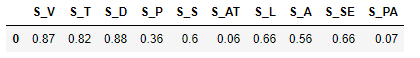
\includegraphics[scale=1.0]{Figures/student_context.PNG}
    \caption{Student context template}
    \label{chap5:sc_template}
\end{figure}

% \subsubsection{Content \label{chap5:content}}

\begin{table}[H]
    \centering
 \begin{tabular}{|p{3.8cm}|p{10.3cm}|} 
    \hline
    \textrm{\textbf{Content Context}} & \textrm{\textbf{Description}} \\ \hline
    \textrm{Ease of understanding (C\_E)} & \textrm{How relatively easy is it to understand the content?}\\ \hline
    \textrm{Simple/Intuition (C\_I)} & \textrm{Does it provide a surface level or deep understanding of the topic?} \\ \hline
    \textrm{Surface/In-depth (C\_ID)} & \textrm{How much preference is given to live experiments to help understand a concept?} \\ \hline
    \textrm{Brief/Concise (C\_C)} & \textrm{Is it short, to the point or descriptive, verbose and elaborative, keeping in mind that learners have different levels of concentration and capacity to remember?} \\ \hline
    \textrm{Thorough (C\_T)} & \textrm{How well does the content item cover the topic?} \\ \hline
    \textrm{Preference/Well reviewed/Well rated(C\_R)} & \textrm{How well rated is the explanation? } \\ \hline
    \textrm{Theoretical/Abstract (C\_A)} & \textrm{How theoretical or abstract is the content item?} \\ \hline
    \textrm{Practical/Hands on (C\_P)} & \textrm{Is it something that can be tried or experienced?} \\ \hline
    \textrm{Experimental/Task-based (C\_ETB)} & \textrm{Does it require a task to be completed to fully understand it, like collaboration with other students or some research/findings?} \\ \hline
    \end{tabular}
    \caption{Content context}
    \label{chap5:content}
\end{table}

% \subsubsection{An Example Data Point \label{chap5:datapoint}}

Below (Figure \ref{chap5:cc_template}) is a content context data point prepared for the course. This content item is thorough(\textit{C\_T}), practical(\textit{C\_P}), and experimentally sound(\textit{C\_ETB}), but not in-depth(\textit{C\_ID}),concise(\textit{C\_C}), and abstract(\textit{C\_A}). It is moderate in terms of  understanding(\textit{C\_E}), intuitiveness(\textit{C\_I}) and has positive reviews(\textit{C\_R}). \par

\begin{figure}[H]
    \centering
    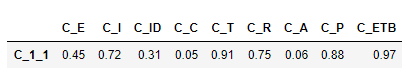
\includegraphics[scale=1.0]{Figures/content_context.PNG}
    \caption{Content context template}
    \label{chap5:cc_template}
\end{figure}

Apart from the above contextual data, there is a course which is taught. For our experiments, we consider a typical course which comprises of topics to be taught. These topics are labeled as \textit{ T\_1, T\_2 ... T\_25}. For e.g: T\_1 refers to the first topic of the course. Each topic has between 5 to 20 different content items. Each content is labeled in the format \textit{C}\_\textit{topic-id}\_\textit{content-number}. For e.g: C\_1\_2 refers to the second content item for topic T\_1. \par

We now have the required contextual information. Topics in the course are taught in a sequence outlined by the teacher. This allows them to control the course sequence. Let us take an example to understand the data.\par

\section{Environment \label{chap5:environment}}

We run a simulation of a course being taken by students with the omniscient policy and the learning algorithm deciding the content item to be presented for each student. It is an environment where several students are taking the course at the same time. Both the omniscient policy and the learning algorithm work in online mode. The learning algorithm updates it's parameters in each round to give better predictions. \par

\section{Evaluation Strategy \label{chap5:evaluationStrategy}}

Since there are no readily available benchmarks to compare our algorithm, we assume there exist an omniscient policy. This policy has optimal parameters to recommend the best arm to pull.  \par

We run the same course with an omniscient policy and the learning algorithm to evaluate our learning algorithm relative to the omniscient policy. The evaluation is conducted with and without skipping. Due to the stochastic nature of a student's feedback both the omniscient policy and the learning algorithm will run for a different number of rounds. However, the total cumulative reward available is the same for both of them. Hence we evaluate them based on cumulative reward accumulated over all rounds. \par 

We simulate the student feedback as a Bernoulli distribution. Here, the probability of success is the maximum expected reward computed by the omniscient policy. This reward for an arm $a$ with optimal parameters $\theta^{*}_{t,a}$ and with context vector $x_{t,a}$ at round $t$ is given by $E[r_{t,a}|\mathbf{x_{t,a}}] = x^{T}_{t,a}\mathbf{\theta^{*}_{t,a}}$. It is passed to the Bernoulli distribution as the probability of reward for the presented content item. Based on the reward received by the learning algorithm the arm parameters are updated to make better decisions in the upcoming rounds. This experiment aims to find how well does our algorithm optimize an arm's parameters to match the omniscient policy. \par

\section{Omniscient Policy \label{chap5:omniscientPolicy}}

This policy knows all the probability distributions. At every step of makes the way the best decision as it knows the true distributions. It does not have to learn anything. It has optimal parameters $\theta^*$ for each arm. Hence it is expected to maximize the cumulative reward.

This policy calculates the expected payoff for each arm $a$ available for a topic. It then selects the arm which has maximum expected payoff. 

\section{Learning Algorithm \label{chap5:learningAlgorithm}}

The learning algorithm can adapt to several students at the same time to present a content item personalized for each student. For every topic, a student is trying to learn it gets the expected payoff for all available content items. It checks whether it should skip to next topic or remain on the current topic. Skipping is activated only if the student gave no reward for a content item presented for the topic. \par

When a student is on a topic, the algorithm presents a content item that could maximize rewards. After working through the content item, the student shares feedback on the content item. If a reward is sent, then this implies that the student understood the concept and can be taken to the next topic. If no reward was sent, then the student may be presented with the next best content item for the same topic or could be moved to the next topic in the course sequence.\par 

Once the student has shared feedback on the content item, the data is sent to train the skip classifier to make a better prediction in forthcoming rounds. \par

\section{Skip Topic \label{chap5:skipTopics}}

The learning algorithm checks with skip topic feature to decide whether or not the content item should be presented for the current topic. Skip topic predicts this by using a student's context along with the estimated payoff for the current topic and the estimated payoff for the next topic in the course sequence. \par

It makes this decision using an online supervised learning stochastic gradient descent classifier with student context along with the estimated payoff of the current and next topic to make a decision. The label for the classifier depends on the reward received for the topic. If a reward was sent then the label is set to 0 or else it is set to 1. Thus the classifier makes use of the feedback sent by all students to recognize common topics and content items that students find difficult so it could make a confident decision. \par

The aim to create skip topic feature is to streamline learning for a student. If a student has been taught a topic once and was not satisfied with it, then there is the option to skip to the next topic or explain the same topic with a different content item. \par

The skip classifier is a linear support vector machine estimator with hinge loss. The estimator is a regularized linear model with stochastic gradient descent (SGD) learning. The gradient of the loss is estimated, each sample at a time and the model is updated along the way with a decreasing learning rate. The regularizer is a penalty added to the loss function that shrinks model parameters towards the zero vector using squared Euclidean norm \cite{scikit-learn}. \par